\section{Introduction}

Concurrent systems are widely spread and its verification is a nontrivial and important problem.
There are a lot of papers that describe concurrent programs behavior via Push Down Systems or Context-Free languages~\cite{gange2015tool, bouajjani2003generic, chaki2006verifying, ModelPDA1}, and our interest is around a \textit{shuffle} of Context-Free Languages (CFL)~\cite{CFLShuffle}.
This languages describe the interleaving of CFLs (or PDA) and look perfect to describe the interleaved behavior of concurrent programs.

First of all we introduce the notion of \textit{shuffle} operation ($\odot$), that can be defined for sequences as follows:
\begin{itemize}
    \item $\varepsilon \odot u = u \odot \varepsilon = {u}$, for every sequence $ u \in \Sigma^*$;
    \item $\alpha_1 u_1 \odot \alpha_2 u_2 = \{\alpha_1 w | w \in (u_1 \odot \alpha_2 u_2) \} \cup \newline
    \{\alpha_2 w | w \in (\alpha_1 u1 \odot u_2 ) \},  \forall \alpha_1, \alpha_2 \in \Sigma$ and $\forall u_1, u_2 \in \Sigma^*$.
\end{itemize}
For example, $"ab" \odot "123" = \{a123b,a1b23, 12ab3, 123ab, etc.\}$.

Shuffle can be extended to languages as $$L_1 \odot L_2 = \bigcup\limits_{u_1\in L_1, u_2\in L_2} u_1 \odot u_2.$$

We can describe required aspects of behavior of functions (or methods, or subsystems) $f_1, f_2 ... f_n$ from our system $\mathcal{S}$ that run concurrently as shuffle of context-free languages $L_{f_1}, L_{f_2} ... L_{f_n}$ generated for each of them.
As a result, language  $\mathcal{L} = L_{f_1} \odot L_{f_2} \odot... \odot L_{f_n}$ describes all possible executions of our system.
If we want to check a correctness of $\mathcal{S}$, then we should check whether $\mathcal{L}$ contains any ``bad execution''.
Let suppose that the set of bad executions can be described by some regular language $R_1$.
Now we should inspect an intersection $\mathcal{L} \cap R_1$ --- its emptiness means that $\mathcal{S}$ can not demonstrate bad behavior.

The idea described above is used in the paper~\cite{stenman2011approximating}. 
As far as shuffled context-free languages are not closed under intersection with the regular one~\cite{CFLShuffle} and the problem of defining either string is in the shuffle of CFL is NP-Complete,
 authors use a context-free approximation of shuffle of CFL and intersect it with error traces, but since the approximation was used this approach didn't found some of known bugs. 

While NP-completeness may looks like death warrant, there are SAT-solvers which deal with NP problems very successfully.
In this paper we show how to reduce emptiness checking of shuffled CFL and finite regular language intersection to SAT.
Our reduction is very native and use some classical parsing techniques.
Generalization for arbitrary regular language is a topic for future research.


\section{Languages Shuffle to SAT}

First, we assume that $ R_1 $ is finite regular language.
This is possible in assumption that the error can usually be detected in the first iterations of the loops,
so at the first step we can approximate general regular language by fixed unrolling of loops.
This assumption is used in bounded model checking~\cite{BMC}.%, but here we use the bound on traces language instead of program language.

Then we appeal to the intuition of shuffle operation.
If the string $J$ is in the language $B \odot C$ then there is a split of $J$ on strings $J_B = b_1 b_2 ... b_k \in B$
and $J_C = c_1 c_2 ... c_k \in C$
such that $b_1 c_1 b_2 c_2 ... b_k c_k = J$ ($b_i, c_i \in (\Sigma^* \cup \varepsilon)$).
Both $J_B$ and $J_C$ are contained in a language of lines $J$ with all possible omissions of terminals.
An example of such language for string "$abc$" is $Y = \{a, b, c, ab, ac, bc, abc, \varepsilon\}$.
We can narrow the shuffled languages $A$ and $B$ to $A\cap Y$ and $B \cap Y$ since this languages still
contain the strings needed to parse $J$.
This reasoning for $J$ can be extended do the automaton $R_1$ since it contains multiple strings
that we want to check for being in shuffle of $L_{f_1} ... L_{f_n}$. 
Thus we consider $ L_{f_i}' = L_{f_i} \cap R_1', i \in 1..n$ --- the finite context-free narrowing of languages $ L_{i}$.
The desired language of strings with omissions is described by an automaton
$R_1'$ --- an transitive-closure of $ R_1 $ with $\varepsilon$-transitions.

Described language narrowing is based on intersection of context-free and regular languages,
and this problem can be solved with use of an algorithm described in paper~\cite{Grigorev}.
This approach is based on Generalised LL (GLL)~\cite{scott2010gll} and utilizes the
Binarized Shared Packed Parse Forest (SPPF)~\cite{brnglr, SPPF}.
Binarized SPPF compresses derivation trees optimally reusing common nodes and subtrees, thus 
utilizing it for parsing forest representation grants worst-case cubic space complexity~\cite{scott2010gll}.

%or

%Binarized Shared Packed Parse Forest (SPPF)~\cite{brnglr, SPPF} compresses derivation trees optimally reusing common nodes and subtrees.
%Version of GLL~\cite{scott2010gll} which utilizes this structure for parsing forest representation achieves worst-case cubic space complexity~\cite{gllParsingTree}.

Binarized SPPF can be represented as a graph in which each node has one of four types described below.
We denote the start and the end positions of substring as $i$ and $j$ respectively, and we call tuple $(i,j)$ an \textit{extension} of a node.

\begin{itemize}
	\item \textbf{Terminal node} with label $(i, T, j)$.
	\item \textbf{Nonterminal node} with label $(i, N, j)$. 
	This node denotes that there is at least one derivation for substring $\alpha=\omega[i..j-1]$ such that $N \Rightarrow^*_G \alpha, \alpha = \omega[i..j-1] $.
	All derivation trees for the given substring and nonterminal can be extracted from SPPF by left-to-right top-down graph traversal started from respective node.     
	\item \textbf{Intermediate node}: a special kind of node used for binarization of SPPF. These nodes are labeled with $(i,t,j)$, where $t$ is a grammar slot.
	\item \textbf{Packed node} with label $(N \rightarrow \alpha, k)$. 
	Subgraph with ``root'' in such node is one possible derivation from nonterminal $N$ in case when the parent is a nonterminal node labeled with $(<\mkern-9mu | \mkern-9mu> (i, N, j))$.
	
\end{itemize}

%An example of SPPF is presented in figure~\ref{SPPF}. We remove redundant intermediate and packed nodes from the SPPF to simplify it and to decrease the size of the structure.
Since the representation of the languages $ L_{f_1}' ... L_{f_n}'$ in a form of SPPF have a high compactness, 
this representation can be used for a generation of compact boolean formula describing the parse forest. This fomula 
can be built via recursive traversal of SPPF. We convert the binary nodes to the conjunction of children, or in case of multiple 
derivations --- alternation. Terminal nodes of the form ($i,a_i,j$) of $m$'th SPPF are to be transformed to bool
variables $(ia_i^mj)$.

In addition to conjunction of formulas describing SPPFs, there are needed an expression to preserve the
shuffle semantics: the terminals .... should be cosen exactly once, this grants the fact that the union of strings results a valid 
path in $R_1$. For the one path $a b c ...$ in $R_1$ and $n$ given SPPFs the formula describing such condition is a 
conjunction of parts $(1a^1 2)\ XOR\ (1a^2 2)\ XOR\ (1a^3 2)\ ...\ (1a^n 2) $ for each terminal.

%fact that the we are searching the set of 
%strings from SPPFs which produce a valid path in automaton $R_1$.  
%Such problem interpretation intuitively defines the rules of the SAT formula generation.~\cite{Grigorev}
%It consists of 2 parts, connected with conjunction. First one is a conjunction of formulas that describe each SPPF.
%Formula describing SPPF 
%\begin{itemize}
%	\item Define the sets of transitions for each language $L_{f_i}'$ with the alternation
%	of formulas $(t_i^1 \& t_i^2 \& ...\& t_i^k)$, where $t_i^1 ... t_i^k$ are transitions of the same set.
%	\item ...
%	\item ...
%\end{itemize}



%An instance of SAT problem is a boolean formula which is checked by solver for satisfiability. 
%Generation of a formula for the problem defined above consists of 2 parts. The first one describe all sets of 
%terminals produced by each of SPPF. It can be generated with recursive traversal of SPPF to 
%preserve the compactness of representation that grants a SPPF structure.

%The second part of the formula defines the relation between the terminals from sets that might be taken prom SPPFs.
%For example, for the case where an automaton $R_1$ is presented as a string $a_1 a_2 a_3...a_k$, the condition
%is following: each terminal $(i,a_i,j)$ should be contained exactly in one of the chosen sets from SPPFs.
%This condition naturaly described by formulas of the form .

To demonstrate an example of formula generation we consider a shuffle of 2 languages 
produced by grammars $G_1: A\rightarrow K\ c;\ K \rightarrow a\ b\ |\ x\ a$ % $G_1: A\rightarrow K\ c;\ K \rightarrow a\ b\ |\ 1\ a$
and $G_2: B \rightarrow x\ y\ z$ %$G_2: B \rightarrow 1\ 2\ 3$
. $A$ and $B$ are start nonterminals.
We want to check for emptiness an intersection of this shuffle with a string $1ab2c3$. 
A finite automaton for transitive closure of this trace shown below.

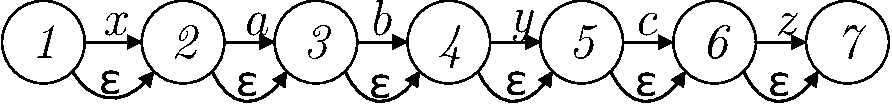
\includegraphics[scale=.54]{./pic/trace2.pdf}

The results of the intersection of languages defined by $G_1$ and $G_2$ are presented as SPPFs in picture
below. Black dots are packed nodes. Note that we removed redundant intermediate and packed nodes from the 
SPPFs to simplify them and to decrease the size of the structure.

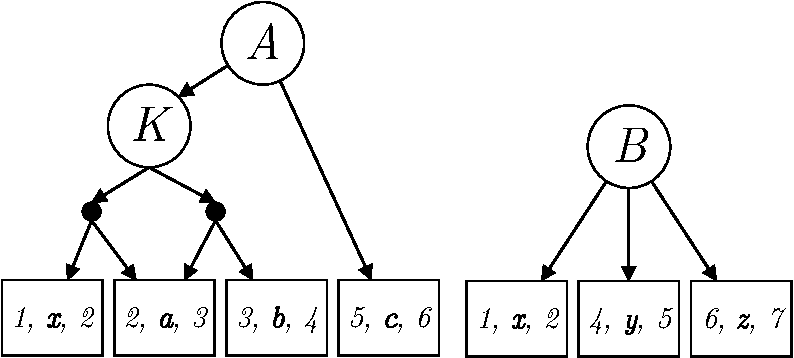
\includegraphics[scale=.6]{./pic/trees2.pdf}


We generate formula $F_1 = (1 x^1 2\ \&\ 2 a^1 3\ |\ 2 a^1 3\ \&\ 3 b^1 4)\ \&\ 5 c^1 6$  % $F_1 = (1 1^1 2\ \&\ 2 a^1 3\ |\ 2 a^1 3\ \&\ 3 b^1 4)\ \&\ 5 c^1 6$ 
for the SPPF for grammar $G_1$
and formula $F_2 = \ 1 x^2 2\ \&\ 4 y^2 5\ \&\ 6 z^1 7$ %$F_2 = \ 1 1^2 2\ \&\ 4 2^2 5\ \&\ 6 3^1 7$
for the second SPPF. Conditions for the 
terminals are described by $F_3 = \ (1 x^1 2\ XOR\ 1 x^2 2)\ \&\ (2 a^1 3\ XOR\ 2 a^2 3)\ \&\ ...\ \&\ (6 z^1 7\ XOR\ 6 z^2 7)$.
%$F_3 = \ (1 1^1 2\ XOR\ 1 1^2 2)\ \&\ (2 a^1 3\ XOR\ 2 a^2 3)\ \&\ ...\ \&\ (6 3^1 7\ XOR\ 6 3^2 7)$.
The final SAT problem is $F_1\&F_2\&F_3$.


%Consider functions Add() and Dec() running concurrently. An \textit{error} operator stands the program reach unwanted state.
%The problem is to define either program can reach the \textit{error} operator. 



%To solve this problem we build Finite Automata to check for an emptiness an intersection $L_prog \cap L_exec$, where
%$L_prog$ is the language described by shuffle of grammars $G_add$ and $G_dec$; $L_exec$ is regular language described by Finite Automaton $R$.


%To preserve the semantics of program we need to add constraints on variables in R.


%then idea is to get formula that describes our intersection. 

%In general, CFG can't be represented by finite SAT formula, because CF grammars can produce infinite 
%lines, thus in model checking widely use bounding of loops and recursion with some N. On the other hand,
%the error traces can be bounded instead of grammars, thus we change our problem to 

%--- 


%Consider such example: we want to define either line $L = a12b3c$ is contained
%in language defined by grammar $S = A \odot B; A = 12 | 123 | a12 | 1a2; B = abc | b3c | 21a$. 

%Let us describe the main ideas of our approach to solve this problem.
%\begin{itemize}
%   \item Generate language $L'$ of all subsequences of $L$, e.g. $L' = \{a, a23, 123, bc, abc, ...\}$.
%   \item Find the intersections of $L'$ with languages of grammars $A$ and $B$. 
%         The results are:
%         \begin{itemize}
%               \item $L'_A = L' \cap L_A = \{12, 123, a12\}$;
%               \item $L'_B = L' \cap L_B = \{abc, b3c\}$.
%         \end{itemize}
%    \item Find a pairs of lines $\{(l'_A, L'_B) : l'_A \in L'_A, L'_B \in L'_B\}$ that can be shuffled to get line $L$. 
%          This pairs are $(123, abc)$ and $(a12, b3c)$. thus we can say that language defined with $G_1$ contains $L$.
%\end{itemize}

%Parsing of regular languages described in~\cite{Grigorev}

\section{Conclusion}

We propose the way to reduce emptiness checking of intersection of shuffled CF languages with finite regular one to SAT.
We show that result formula has a special structure (huge XOR subformula) which require to use XOR-SAT-solvers.
We hope that our restriction on regular language is week enough to solve real tasks.
To prove it it is necessary to evaluate our approach on real project.

Main question for future research is decidability of emptiness of shuffled CFL and regular language intersection.
It is known that shuffled CFL is not closed under intersection with regular languages~\cite{CFLShuffle}, but decidability of intersection emptiness is looks an open question.
If it will be shown that it is undecidable in general case, then it is interesting to find subclasses for which this problem is decidable.



\begin{acks}
The research was supported by the Russian Science Foundation grant 18-11-00100 and a grant from JetBrains Research.   
\end{acks}
